% file: modeledsystems.tex

\chapter{Modeled systems}
The goal of this thesis is to study fracture of methane hydrates. In order to do that, I need to know the mechanical properties of the model I study. Since studies of mechanical properties of methane hydrates modeled with TIP4P/ICE+UAM are scarce, I start this chapter by working out even the basic mechanical properties such as Poissons ratio and Youngs modulus. In order to be sure that the methods I use to estimate the mechanical properties work, I first check them with known values for a Lennard-Jones crystal. 

\section{Shear viscosity and diffusivity}
I have not been successful in finding values for the shear viscosity and diffusivity of bulk liquid water modeled with TIP4P/ICE. To measure these properties, I run a simulation like the one I ran to calculate verify the same properties for the TIP4P/2005 potential. Figure @ref shows the Green-Kubo relation for the viscosity using 5 independent pressure components. The shear viscosity is estimated to $\eta_{GK} = \text{\SI{1.63\pm 0.05}{\milli\pascal\second}}$. 

\begin{figure}
\centering
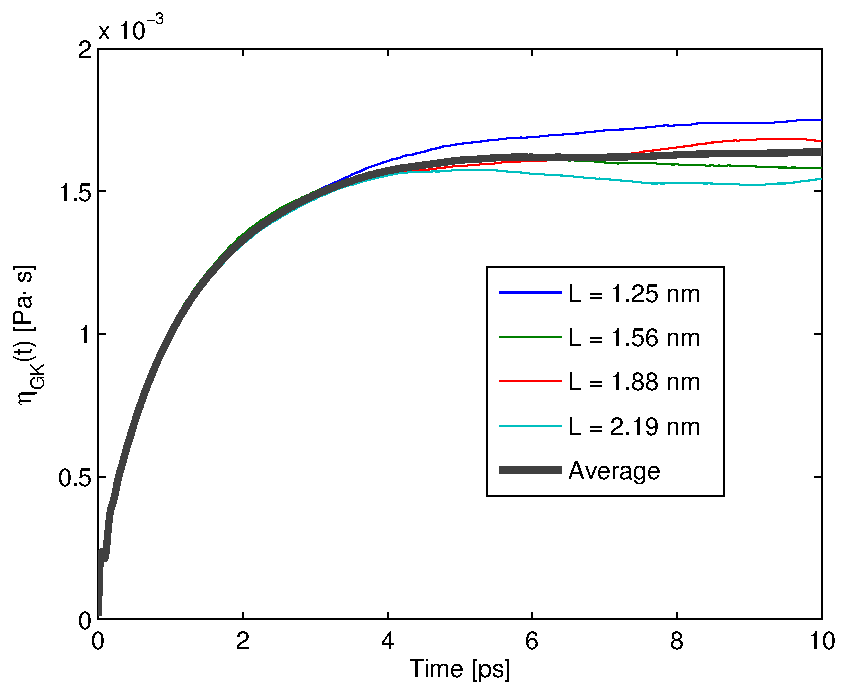
\includegraphics[width=10cm]{../figures/thesis/viscosity_green_kubo_tip4p_ice.pdf}
\caption{Shear viscosity for TIP4P/ICE at \SI{300}{\kelvin} and $\rho = \text{\SI{0.98}{\gram\per\cubic\cm}}$. The viscosity is estimated to $\eta_{GK} = \text{\SI{1.63\pm0.05}{\milli\pascal\second}}$}
\end{figure}

\section{Measuring elastic properties with a constand strain rate}
A naive approach, which i will use for crude estimates, is to subject a system to a constant strain rate by expanding the simulation box in one of the coordinate directions, and rescale all atom positions accordingly. An anisotropic thermo-barostat should be applied along the other axes, to keep the environment pressure and temperature constant. Since the barostat scales the simulation box, strains along the two axes perpendicular to the applied strain can be measured as the contraction of the simulation box in these directions:

\begin{equation}
\varepsilon_i = \frac{L_i-L_{0, i}}{L_{0, i}}
\end{equation}

If the sample is isotropic, I only have to simulate strain application in one of the coordinate directions to estimate both Young's modulus and Poissons ratio for a given system. To account for the possibility that the model I use do not exhibit isotropic behavior, I will check strains in both of the coordinate axes that are perpendicular to the axis of applied strain when calculating Poissons ratio. The scalar value of $\nu$ is the slope of the strain-strain curve, and for $E$ of the stress-strain curve, both in their linear regions. I will calculate these slopes using linear regression with least squares on the curves.
In the following, I will apply the method described above to a Lennard-Jones crystal and to the TIP4P/ICE+UAM methane hydrate model.

\subsection{Lennard-Jones crystal}
The FCC-lattice with a Lennard-Jones potential has been extensively investigated due to its simplicity. Therefore it provides robust benchmarking capabilities. I want to check that my protocols for dynamic (but quasistatic) determination of elastic properties and fracture strength reproduces known parameters for a Lennard-Jones solid. Reference values are for Young's modulus, $E=61.1 \epsilon/\sigma^3 = \text{\SI{2.40}{\giga\pascal}}$ (for the parameters I use for Methane), and for Poissons ratio, $\nu=0.347$. Values are taken from a molecular dynamics study by Quesnel et al. \cite{Quesnel1993}.

Figures \ref{fig:stress_strain_11_11_11_and_22_22_22_y_z_poisson_lennard_jones} and \ref{fig:strain_strain_11_11_11_and_22_22_22_y_z_poisson_lennard_jones} show data for a strain test of two systems of Lennard-Jones particles subjected to a strain rate of \SI{2d-8}{\per\femto\second} over \SI{0.8}{\nano\second} resulting in a maximum strain of \SI{0.8}{\percent}. The external pressure was set to \SI{50}{\mega\pascal}, and the temperature was \SI{5}{\kelvin}. Along with the data are estimates of Poissons ratio and Young's modulus, taken as the best linear regression with least squares. 


\begin{figure}
\centering
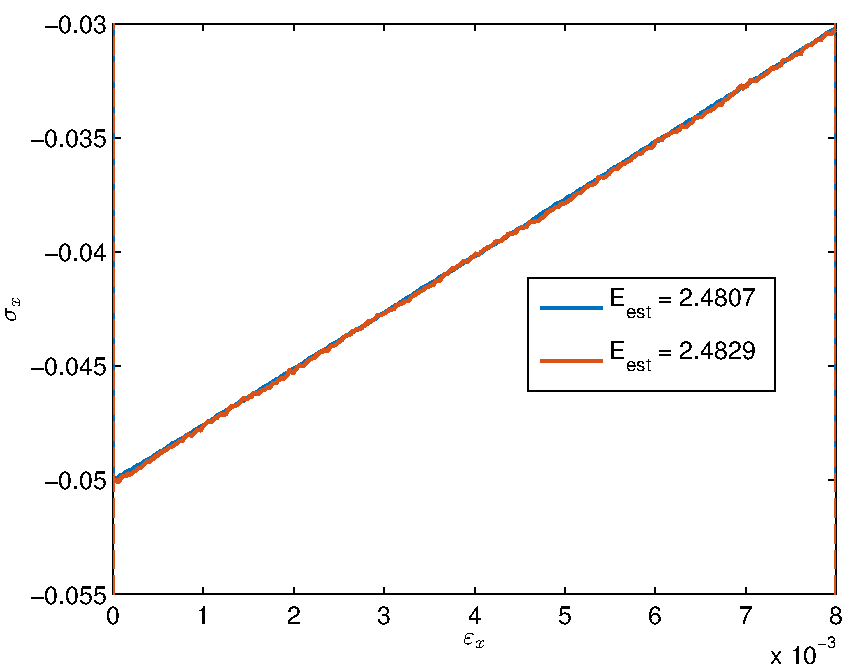
\includegraphics[width=10cm]{../figures/thesis/stress_strain_11_11_11_and_22_22_22_y_z_poisson_lennard_jones.pdf}
\caption{Stress-strain relations for Lennard-Jones systems of $11^3$ (red) and $22^3$ (blue) FCC unit cells. The sample was subjected to a constant strain rate of \SI{2d-8}{\per\femto\second}. $E$ is estimated using linear regression with least squares on all data points.}
\label{fig:stress_strain_11_11_11_and_22_22_22_y_z_poisson_lennard_jones}
% Path to simulation: /media/henriasv/Data/molecular-data/master_methane_hydrates/stress_strain/20150113_lennard_jones_strain
\end{figure}

\begin{figure}
\centering
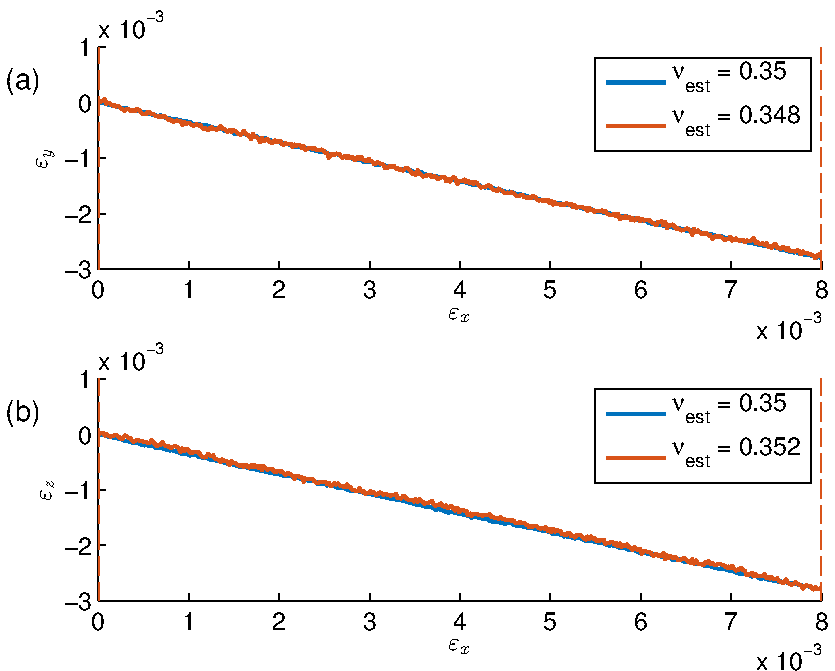
\includegraphics[width=10cm]{../figures/thesis/strain_strain_11_11_11_and_22_22_22_y_z_poisson_lennard_jones.pdf}
\caption{Strain-strain relations for for the same simulations as in Figure \ref{fig:stress_strain_11_11_11_and_22_22_22_y_z_poisson_lennard_jones}. All data points were used to estimate $\nu$.}
\label{fig:strain_strain_11_11_11_and_22_22_22_y_z_poisson_lennard_jones}
% Path to simulation: /media/henriasv/Data/molecular-data/master_methane_hydrates/stress_strain/20150113_lennard_jones_strain
\end{figure}

\subsection{S1 methane hydrate with TIP4P/ICE+UAM}
To my knowledge, there are no published estimates of Youngs modulus and the Poisson ratio for the TIP4P/ICE+UAM model of methane hydrates. Therefore, I seek to make crude estimates of these quantities in dynamic simulations. I apply a constant strain rate by continously rescaling particle positions in one direction during MD-simulations. The other directions are kept under a constant pressure with anisotropic barostatting.
Figure \ref{fig:stress_strain_11_11_11_tip4p_ice_uam} shows the stress strain relationships and corresponding estimates of Youngs modulus for a system of 11x11x11 S1 unit cells subjected to strain rates of \SI{5d-7}{\per\femto\second} and \SI{2d-7}{\per\femto\second}. By extrapolating the results to quasistatic strain, Youngs modulus is estimated to \SI{7.1}{\giga\pascal}. 
Figure \ref{fig:strain_strain_11_11_11_y_z_poisson_tip4p_ice_uam} shows the relationship between applied strain along the x-axis and the measured strain along the other axes. It is not outrageous to assume S1 methane hydrate to be isotropic. Under this assumption, and by extrapolation to quasisatic strain, I estimate the poisson ratio for this model of S1 methane hydrate to be $\nu = 0.41$. 

\begin{figure}
\centering
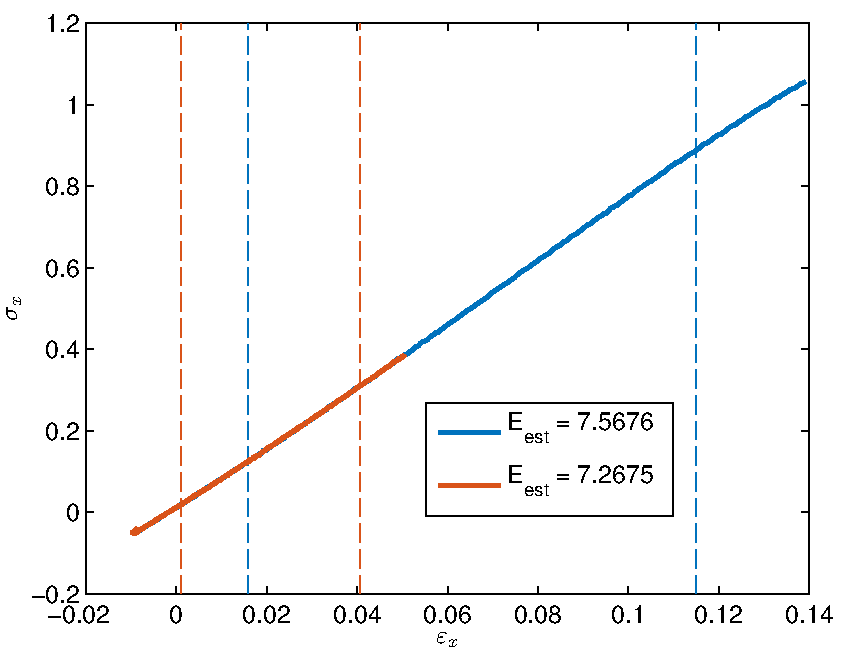
\includegraphics[width=10cm]{../figures/thesis/stress_strain_11_11_11_tip4p_ice_uam.pdf}
\caption{Stess-strain relations for a system of 11x11x11 S1 unit cells. Dashed lines indicate the region that was used to estimate Youngs modulus. Strain rates of \SI{5d-7}{\per\femto\second} (blue) and \SI{2d-7}{\per\femto\second} (red) along the x-axis.}
\label{fig:stress_strain_11_11_11_tip4p_ice_uam}
% Path to simulation: /media/henriasv/Data/molecular-data/master_methane_hydrates/stress_strain/20150108_youngs_modulus

\end{figure}

\begin{figure}
\centering
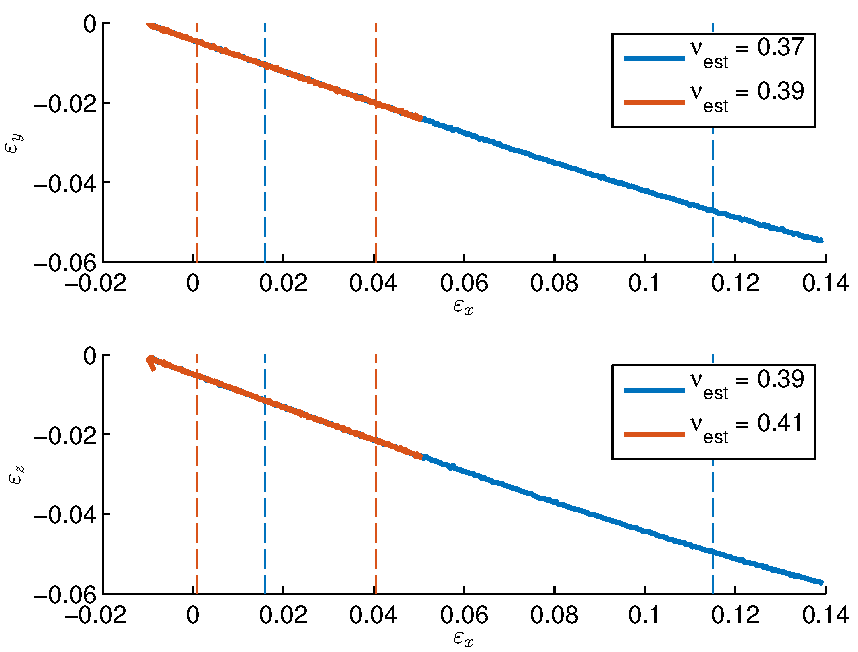
\includegraphics[width=10cm]{../figures/thesis/strain_strain_11_11_11_y_z_poisson_tip4p_ice_uam.pdf}
\caption{Strain-strain relations for the same system as in Figure \ref{fig:stress_strain_11_11_11_tip4p_ice_uam}. Measured strain along the y-axis (a) and z-axis (b) is plotted against the applied strain along the x-axis. Dashed lines indicate the region that was used to estimate Poissons ratio.}
\label{fig:strain_strain_11_11_11_y_z_poisson_tip4p_ice_uam}
% Path to simulation: /media/henriasv/Data/molecular-data/master_methane_hydrates/stress_strain/20150108_youngs_modulus

\end{figure}

\section{Fracture and fracture toughness}

\subsection{Determining the critical stress intensity factor}
As described in the section about fracture mechanics, the stress intensity factor is commonly used to calculate the fracture toughness of a material. Assuming methane hydrates to be brittle (which jush might be a good assumption), I use fracture theories developed by Griffiths to estimate the stress intensity factor for S1 methane hydrate. I cut a 

\section{Vega 2010}

